%style


\newcommand{\views}{\mathsf{views}}

\pagestyle{fancy}

\newcommand{\period}{.}%used in equations
\newcommand{\comma}{,}%used in equations

\newcommand{\tn}[1]{#1}% a number which is inlined in the text, and could be replaced by a word, e.g.
%has length at most \tn{3}
\newcommand{\an}[1]{$#1$}% a number which is inlined in the text, but represents an alphabet symbol,
%e.g. the set of words in which the number of \an{1}'s and \an{0}'s are equal.

%shrink bullets
\newlength{\mylen}
\newlength{\itemizemargin}%leftmargin for itemize lists
\newlength{\itemizelabelsep}%labelsep for itemize lists
\setbox1=\hbox{$\bullet$}\setbox2=\hbox{\tiny$\bullet$}
\setlength{\mylen}{\dimexpr0.5\ht1-0.5\ht2}
\setlength{\itemizemargin}{27pt}
\setlength{\itemizelabelsep}{\dimexpr 0.4\itemizemargin}
\renewcommand\labelitemi{\raisebox{\mylen}{\tiny$\bullet$}}
\renewcommand\labelitemii{\raisebox{\mylen}{\tiny$\bullet$}}
\setlist[itemize]{leftmargin=\itemizemargin,labelsep=\itemizelabelsep}

\newcommand{\tagsymbol}{$\diamond$}


\DeclareTextFontCommand{\textsmallcaps}{\scshape}

      \RequirePackage{letterspace}
      \RequirePackage{textcase}
      % Set up letterspacing (using microtype package) -- requires pdfTeX v1.40+
      \newcommand{\allcapsspacing}[1]{\textls[200]{#1}}
      \newcommand{\smallcapsspacing}[1]{\textls[50]{#1}}
      \newcommand{\allcaps}[1]{\textls[200]{\MakeTextUppercase{#1}}}
      \newcommand{\smallcaps}[1]{\smallcapsspacing{\scshape\MakeTextLowercase{#1}}}
      \renewcommand{\textsc}[1]{\smallcapsspacing{\textsmallcaps{#1}}}

\newcommand{\newlinetospace}[1]{#1}
% \DeclareRobustCommand{\newlinetospace}[1]{%
%   \let\@tufte@orig@cr\\% save the original meaning of \\
%   \def\\{\@tufte@newlinetospace}% turn \\ and \\* into \space
%   \let\newline\\% turn \newline into \space
%   #1%
%   \let\\\@tufte@orig@cr% revert to original meaning of \\
% }

\makeatletter
\newcommand*{\currentname}{\@currentlabelname}


\newcommand\iraggedright{%ragged right with indentation
  \let\\\@centercr\@rightskip\@flushglue \rightskip\@rightskip
  \leftskip\z@skip}



\newboolean{@test@}%if true, only parts encompassed in environment testshow will be typeset.
\setboolean{@test@}{true}

\newcommand{\testhide}[1]{
\ifthenelse{\boolean{@test@}}{}{#1}%in test mode contents is hidden
}


\newboolean{@tufte@symmetric}
\setboolean{@tufte@symmetric}{true}
\newboolean{@tufte@twoside}
\setboolean{@tufte@twoside}{true}


% The running heads/feet don't have rules
\renewcommand{\headrulewidth}{0pt}
\renewcommand{\footrulewidth}{0pt}
\newcommand{\plaintitle}{}
\newcommand{\plainauthor}{}
\setlength{\headsep}{45pt}
% The 'fancy' page style is the default style for all pages.
\fancyhf{} % clear header and footer fields
\newcommand{\headdisplay}[1]{{\fontsize{6.5}{0}\fontseries{b}\selectfont\scshape\textls[150]{#1}}}
\fancyhead[LE]{\thepage\quad\headdisplay{\leftmark}}%
\fancyhead[RO]{\headdisplay{\rightmark}\quad\thepage}


\renewcommand{\chaptermark}[1]%
   {\markboth{\MakeUppercase{#1}}{}}
\renewcommand{\sectionmark}[1]%
   {\markright{\MakeUppercase{#1}}}


\newlength{\@tufte@overhang}% used by the fullwidth environment and the running heads
\newlength{\@tufte@fullwidth}
\newlength{\@tufte@caption@fill}

\newcommand{\TufteRecalculate}{%
  \setlength{\@tufte@overhang}{\marginparwidth}
  \addtolength{\@tufte@overhang}{\marginparsep}

  \setlength{\@tufte@fullwidth}{\textwidth}
  \addtolength{\@tufte@fullwidth}{\marginparsep}
  \addtolength{\@tufte@fullwidth}{\marginparwidth}

  \setlength{\@tufte@caption@fill}{\textwidth}
  \addtolength{\@tufte@caption@fill}{\marginparsep}
}

\AtBeginDocument{\TufteRecalculate}
% Set the header/footer width to be the body text block plus the margin
% note area.
% \AtBeginDocument{%
%   \ifthenelse{\boolean{@tufte@symmetric}}
%     {\fancyhfoffset[LE,RO]{\@tufte@overhang}}
%     {\fancyhfoffset[RE,RO]{\@tufte@overhang}}
% }


\RequirePackage{titlesec,titletoc}
%%
% Make Tuftian-style section headings and TOC formatting

\titleformat{\part}%
  [display]% shape
  {\relax\ifthenelse{\NOT\boolean{@tufte@symmetric}}{\begin{fullwidth}}{}}% format applied to label+text
  {}%{\scshape \LARGE part\ \thepart\\}% label
  {0pt}% horizontal separation between label and title body
  {\Huge\rmfamily\itshape}% before the title body
  [\ifthenelse{\NOT\boolean{@tufte@symmetric}}{\end{fullwidth}}{}]% after the title body

\titleformat{\chapter}%
  [display]% shape
  {\relax\ifthenelse{\NOT\boolean{@tufte@symmetric}}{\begin{fullwidth}}{}}% format applied to label+text
  {\itshape\huge\thechapter}% label
  {0pt}% horizontal separation between label and title body
  {\huge\rmfamily\itshape}% before the title body
  [\ifthenelse{\NOT\boolean{@tufte@symmetric}}{\end{fullwidth}}{}]% after the title body


\titleformat{\section}%
  [hang]% shape
  {\normalfont\Large\itshape}% format applied to label+text
  {\normalfont\Large\itshape\thesection}% label
  {1em}% horizontal separation between label and title body
  {}% before the title body
  []% after the title body

\titlespacing*{\chapter}{0pt}{50pt}{40pt}
\titlespacing*{\section}{0pt}{3.5ex plus 1ex minus .2ex}{2.3ex plus .2ex}
\titlespacing*{\subsection}{0pt}{3.25ex plus 1ex minus .2ex}{1.5ex plus.2ex}


%%
% When \cleardoublepage is called, produce a blank (empty) page -- i.e.,
% without headers and footers
\def\cleardoublepage{\clearpage\if@twoside\ifodd\c@page\else
  \hbox{}
  %\vspace*{\fill}
  %\begin{center}
  %  This page intentionally contains only this sentence.
  %\end{center}
  %\vspace{\fill}
  \thispagestyle{empty}
  \newpage
  \if@twocolumn\hbox{}\newpage\fi\fi\fi}

%%
% Set the font sizes and baselines to match Tufte's books
\renewcommand\normalsize{%
   \@setfontsize\normalsize\@xpt{14}%
   \abovedisplayskip 10\p@ \@plus2\p@ \@minus5\p@
   \abovedisplayshortskip \z@ \@plus3\p@
   \belowdisplayshortskip 6\p@ \@plus3\p@ \@minus3\p@
   \belowdisplayskip \abovedisplayskip
   \let\@listi\@listI}
\normalbaselineskip=14pt
\normalsize
\renewcommand\small{%
   \@setfontsize\small\@ixpt{12}%
   \abovedisplayskip 8.5\p@ \@plus3\p@ \@minus4\p@
   \abovedisplayshortskip \z@ \@plus2\p@
   \belowdisplayshortskip 4\p@ \@plus2\p@ \@minus2\p@
   \def\@listi{\leftmargin\leftmargini
               \topsep 4\p@ \@plus2\p@ \@minus2\p@
               \parsep 2\p@ \@plus\p@ \@minus\p@
               \itemsep \parsep}%
   \belowdisplayskip \abovedisplayskip
}
\renewcommand\footnotesize{%
   \@setfontsize\footnotesize\@viiipt{10}%
   \abovedisplayskip 6\p@ \@plus2\p@ \@minus4\p@
   \abovedisplayshortskip \z@ \@plus\p@
   \belowdisplayshortskip 3\p@ \@plus\p@ \@minus2\p@
   \def\@listi{\leftmargin\leftmargini
               \topsep 3\p@ \@plus\p@ \@minus\p@
               \parsep 2\p@ \@plus\p@ \@minus\p@
               \itemsep \parsep}%
   \belowdisplayskip \abovedisplayskip
}
\renewcommand\scriptsize{\@setfontsize\scriptsize\@viipt\@viiipt}
\renewcommand\tiny{\@setfontsize\tiny\@vpt\@vipt}
\renewcommand\large{\@setfontsize\large\@xipt{15}}
\renewcommand\Large{\@setfontsize\Large\@xiipt{16}}
\renewcommand\LARGE{\@setfontsize\LARGE\@xivpt{18}}
\renewcommand\huge{\@setfontsize\huge\@xxpt{30}}
\renewcommand\Huge{\@setfontsize\Huge{24}{36}}

\makeatother


\renewcommand\qedsymbol{\scalebox{0.75}{$\blacksquare$}}

\fancypagestyle{plain}{
  \fancyhf{} % clear header and footer fields
  % Uncomment the following five lines of code if you want the opening page
  % of the chapter to express the folio in the lower outside corner.
  %\ifthenelse{\boolean{@tufte@twoside}}
  %  {\fancyfoot[LE,RO]{\thepage}}
  %  {\fancyfoot[RE,RO]{\thepage}}
}


  \titlecontents{part}%
    [3em] % distance from left margin
{\addvspace{3pt}\vspace{1.5\baselineskip}\LARGE\bfseries\itshape} % above (global formatting of entry)
    {\hspace*{0em}\contentslabel{2em}} % before w/label (label = ``2'')
    {\hspace*{0em}} % before w/o label
    {\rmfamily\upshape\qquad\thecontentspage} % filler + page (leaders and page num)
    [\vspace{5pt}] % after


  \titlecontents{chapter}%
    [3em] % distance from left margin
{\addvspace{3pt}\vspace{1.5\baselineskip}\LARGE\rmfamily\itshape} % above (global formatting of entry)
    {\hspace*{0em}\contentslabel{2em}} % before w/label (label = ``2'')
    {\hspace*{0em}} % before w/o label
    {\rmfamily\upshape\qquad\thecontentspage} % filler + page (leaders and page num)
    [\vspace{5pt}] % after

  \titlecontents{section}% FIXME
    [3em] % distance from left margin
    {\vspace{5pt}\vspace{0\baselineskip}\Large\rmfamily\itshape} % above (global formatting of entry)
    {\hspace*{2em}\contentslabel{2em}} % before w/label (label = ``2.6'')
    {\hspace*{2em}} % before w/o label
    {\rmfamily\upshape\qquad\thecontentspage} % filler + page (leaders and page num)
    [\addvspace{3pt}] % after

% (margin) notes 
%
\newcommand{\todonote}[2]{\todo[inline]{{\bf (#1)}: #2}}
\newcommand{\igw}[1]{\todo[size=\tiny,fancyline,color=blue!30]{{\bf (igw)}: #1}}
\newcommand{\ms}[1]{\todonote{MS}{#1}}
\newcommand{\sla}[1]{\todo[size=\tiny,fancyline,color=green!40]{{\bf (SL)}: #1}}
\newcommand{\slaInlini}[1]{\todonote{SL}{#1}}
\newcommand{\pawel}[1]{\todo[size=\tiny,fancyline,color=green!40]{{\bf (PP)}: #1}\xspace}
\newcommand{\henryk}[1]{\todo[size=\tiny,fancyline,color=orange!40]{{\bf (HM)}: #1}}
\newcommand{\sz}[1]{\todo[size=\tiny,fancyline,color=blue!40]{{\bf (sz)}: #1}}
\newcommand{\fmu}[1]{\todo[size=\tiny,fancyline,color=red!40]{{\bf (FMu)}: #1}}
\newcommand{\fma}[1]{\todo[size=\tiny,fancyline,color=purple!40]{{\bf (FMa)}: #1}}
\newcommand{\shu}[1]{\todo[size=\tiny,fancyline,color=green!40]{{\bf (SH)}: #1}}
\newcommand{\shuInlini}[1]{\todonote{SH}{#1}}
\newcommand{\eryx}[1]{\todo[size=\tiny,fancyline,color=green!40]{{\bf (EK)}: #1}}
%\newcommand{\wojtek}[1]{\todo[size=\tiny,fancyline,color=green!40]{{\bf (WC)}: #1}}
\newcommand{\wojtek}[1]{}

\newcommand{\mipi}[1]{\todo[size=\tiny,fancyline,color=blue!20]{{\bf (MiPi)}: #1}}
\newcommand{\klin}[1]{\todo[size=\tiny,fancyline,color=olive!20]{{\bf (BK)}: #1}}
\newcommand{\lorenzo}[1]{\todo[size=\tiny,fancyline,color=green!40]{{\bf (LC)}: #1}}
\newcommand{\joost}[1]{\todo[size=\tiny,fancyline,color=purple!40]{{\bf (JW)}: #1}}
\newcommand{\lorenzolong}[1]{\todonote{Wawrzyniec}{#1}}

% (SL) general
%
% star exercise
\newcommand{\starmark}{{\normalfont \upshape{\raisebox{0pt}{$(\ast)$}}}}
\newcommand{\starexercise}{\noindent \starmark\ }
% hint
\newcommand{\hint}[1]{\smallskip \noindent \smallcaps{Hint:}{\slshape\ #1}}
\newcommand{\note}{\smallskip \noindent \smallcaps{Note:}\ } %SH
% empty word
\newcommand{\emptyword}{\varepsilon}
% unified way of defining sets
\newcommand{\setof}[2]{\left\{#1 \,\mid\, #2 \right\}}
\newcommand{\set}[1]{\{#1\}}
% powerset
\newcommand{\powerset}[1]{{\cal P}(#1)}
% length of a word
\newcommand{\len}[1]{\lvert #1 \rvert}


\newcommand{\Nat}{\ensuremath{\mathbb{N}}}
\newcommand{\Int}{\ensuremath{\mathbb{Z}}}

\newcommand{\problemtitle}[1]{\smallcaps{#1}}
%some problems have titles, 
%which appear immediately at the beginning

%% math symbols

\newcommand{\unaryplus}{\raisebox{0.5pt}{\scalebox{0.65}{\( + \)}}}
\newcommand{\unaryminus}{\raisebox{0.5pt}{\scalebox{0.65}{\( - \)}}}
\newcommand{\cinc}{\unaryplus\unaryplus}%counter increment
\newcommand{\cdec}{\unaryminus\unaryminus}%counter decrement

%% math operators

\renewcommand\bar[1]{\overline{#1}}


% left composition symbol (Z notation)
%\DeclareMathSymbol{\fcmp}{\mathrel}{bbold}{\lq\;}
\newcommand{\fcmp}{\cdot}


% (SH)
\newcommand{\yesmark}{\checkmark}
\newcommand{\nomark}{\ensuremath{\times}\xspace}
% (SH)
\newcommand{\pairletter}[2]{\bigg[{{#1}\atop{#2}}\bigg]} 


%(Sz T) 
%uniformize set difference and inclusion
\renewcommand{\subset}{\subseteq}
\renewcommand{\setminus}{-}
% (FMu) disjoint union
\newcommand{\disunion}{+}

%the set of all infixes of a language L: \infixes L
\newcommand{\infixes}{\text{Infixes}}

%context-free grammar notation. Example: S\produce Sa \sep Sb \sep \emptyword
\newcommand{\produce}{\rightarrow}
\newcommand{\sep}{\mathop{\big|}}

%Pumping lemma notation: a long word in a context-free language decomposes as \prefix \pleft \infix \pright \suffix
\newcommand{\prefix}{\mathit{prefix}}
\newcommand{\infix}{\mathit{infix}}
\newcommand{\suffix}{\mathit{suffix}}
\newcommand{\pleft}{\mathit{left}}
\newcommand{\pright}{\mathit{right}}


\newcommand{\hatphi}{\widehat{\varphi}}
\newcommand{\hatgamma}{\widehat{\gamma}}

\newcommand{\leftpar}{\texttt{\upshape(}}
\newcommand{\rightpar}{\texttt{\upshape)}}
% (SL) Turing machines terminology
%
\newcommand{\initstate}{q_0}
\newcommand{\accstate}{q_f}
\newcommand{\blanksymb}{\textsc{b}}
\newcommand{\states}{Q}
\newcommand{\alphabet}{\Sigma}
\newcommand{\tapealphabet}{T}
\newcommand{\lewo}{\leftarrow}
\newcommand{\tutaj}{\circlearrowleft}
\newcommand{\prawo}{\rightarrow}
\newcommand{\transrules}{\delta}
% (SH)
\newcommand{\markend}{\$}

% (MS) ignore
\newcommand{\ignore}[1]{}

% (MS) Vertical letter with two coordinates
% i.e. \vletterab{a}{b} gives [a/b]
\newcommand{\vletterab}[2]{\left[\hspace{-5pt}\begin{array}{c} {#1} \\ {#2} \end{array}\hspace{-5pt}\right]}

% (MS) Vertical letter with three coordinates
% i.e. \vletterabc{a}{b}{c} gives [a/b/c]
\newcommand{\vletterabc}[3]{\left[\hspace{-5pt}\begin{array}{c} {#1} \\ {#2} \\ {#3} \end{array}\hspace{-5pt}\right]}

% (MS) A function
% i.e. \fun{f}{X}{Y} gives f : X -> Y
\newcommand{\fun}[3]{#1\colon #2 \to #3}

% (MS) A partial function
% i.e. \parfun{f}{X}{Y} gives f : X -' Y
\newcommand{\parfun}[3]{#1\colon #2 \rightharpoonup #3}

% (MS) A transition of an automaton
% i.e. p \tran{a} q
\newcommand{\tran}[1]{\xrightarrow{#1}}

% (MS) The equational symbol of definition
% i.e. L^n \eqdef L\cdot L \cdot\ldots \cdot L
%\newcommand{\eqdef}{\stackrel{\text{def}}=}

% (MS) The comprehension scheme symbol
% i.e. \{ w \mid w^2 \in L \}
\renewcommand{\mid}{:}

% (MS) The star in regular expressions
% i.e. w*\ast, \Sigma^\ast, L^\ast etc.
\renewcommand{\ast}{{*}}

% (MS) The plus in regular expressions
% i.e. w*\plus, \Sigma^\plus, L^\plus etc.
\newcommand{\plus}{{+}}

% (MS) The symbol used to reverse words and languages,
% i.e. L^\rev or w^\rev
\newcommand{\rev}{\mathrm{R}}

% (SH) operation of reversing
% i.e. \rev{L} or \rev{w}
\newcommand{\revop}[1]{{#1}^{\rev}}

% (MS) The operation constructing the cycled language:
% \cycle(L) = \{ uv : vu \in L \}
\newcommand{\cycle}{\mathrm{Cycle}\xspace}

% (FMu) The number of occurrences of word u in word w
% i.e. \occ{u,w}
\newcommand{\occ}[2]{\#_{#1}(#2)}


% (FMu) The automata font 
\newcommand{\aut}[1]{{\mathcal{#1}}}


% (MS) The set of non-trivial palindromes over a given alphabet
% i.e. \Pal_\Sigma = \{ u : u = u^\rev \wedge |u| \geq 2 \}
\newcommand{\Pal}{\mathrm{Pal}\xspace}

% (MS) The binary evaluation map \bin \colon \{0,1\}^* \to [0,1]
% i.e. \bin(101) = 0.625
\newcommand{\bin}{\mathrm{bin}\xspace}

% (WC)
% lowest common multiplicity
\newcommand{\lcm}{\mathrm{lcm}\xspace}
% label of the run
\newcommand{\lab}{\mathrm{lab}\xspace}
% size
\newcommand{\size}{\mathrm{size}}


%\renewcommand{\O}{\mathcal{O}}
\newcommand{\rank}{\mathit{rank}}
\newcommand{\floor}[1]{\lfloor #1 \rfloor}

\newcommand{\A}{\mathcal{A}}
\newcommand{\N}{\mathbb{N}}
\newcommand{\Z}{\mathbb Z}
\newcommand{\Q}{\mathbb Q}
\newcommand{\R}{\mathbb R}
\renewcommand{\P}{\mathbb P}
\newcommand{\E}{\mathbb E}
\newcommand{\F}{\mathcal F}
\newcommand{\G}{\mathcal G}
\renewcommand{\O}{\mathcal O}
\newcommand{\atoms}{\mathbb A}
\newcommand{\diff}{\textup{diff}}
\renewcommand{\inf}{\textup{inf}}
\newcommand{\xor}{\textup{inf-xor}}
\newcommand{\fxor}{\textup{fin-xor}}
\newcommand{\win}{\textup{Win}}
\newcommand{\attr}{\textup{attr}}
%\newcommand{\rank}{\textup{rank}}
\newcommand{\val}{\textup{val}}
%\newcommand{\len}{\textup{len}}
\newcommand{\first}{\textup{first}}
\newcommand{\last}{\textup{last}}
\newcommand{\nextpos}{\textup{next}}
\newcommand{\son}{\textup{son}}
\newcommand{\lson}{\textup{lson}}
\newcommand{\rson}{\textup{rson}}
\newcommand{\desc}{\textup{desc}}
\newcommand{\reach}{\textup{Reach}}
\newcommand{\tw}{\textup{tw}}
\newcommand{\minor}{\trianglelefteq}
\newcommand{\eso}{\exists\text{SO}}

% grammars terminology
%
% (SH) terminals (alphabet)
\newcommand{\terminals}{\Sigma} %TODO: dalem tak dla kompatybilnosci z tekstem Igora, ale mysle, ze powinno byc ujednolicone z \alphabet Slawka, czyli \newcommand{\terminals}{\alphabet}
% (SH) nonterminals (variables)
\newcommand{\nonterminals}{V}
% (SH) initial symbol
\newcommand{\initsymbol}{S}
% (SH) nonterminal associated with a terminal
\newcommand{\nontermletter}[1]{\fbox{$#1$}}
% (SH) nonterminal associated with a terminal that stores a state of a simulated automaton
%\newcommand{\nontermletterst}[2]{{#1}_{#2}}
% (SH) a leter with the word-end-marker
\newcommand{\letterend}[1]{#1^{\markend}}

\def\btrue{\textit{true}\xspace}
\def\bfalse{\textit{false}\xspace}
\renewcommand{\iff}{\Leftrightarrow}


% (MiPi) Complexity classes
\newcommand{\cmpclass}[1]{\smallcaps{#1}}
\newcommand{\cP}{\cmpclass{P}}
\newcommand{\cNP}{\cmpclass{NP}}
\newcommand{\cPSPACE}{\cmpclass{PSPACE\xspace}}
\newcommand{\cNPSPACE}{\cmpclass{NPSPACE\xspace}}
\newcommand{\cL}{\cmpclass{L}}
\newcommand{\cNL}{\cmpclass{NL}}

%TEXT
\newcommand{\leftmost}{left-most\xspace}
\newcommand{\rightmost}{right-most\xspace}

%%% FMu: quick and dirty aligning macro
\newcommand{\fantom}[1]{\textcolor{white}{#1}}

\newcommand{\zloty}{{\textsc{pln}}}
\newcommand{\euro}{{\textsc{eur}}}


%% Caligraphic

\newcommand{\Aa}{\mathcal{A}}
\newcommand{\Bb}{\mathcal{B}}
\newcommand{\Cc}{\mathcal{C}}
\newcommand{\Dd}{\mathcal{D}}
\newcommand{\Ee}{\mathcal{E}}
\newcommand{\Ff}{\mathcal{F}}
\newcommand{\Gg}{\mathcal{G}}
\newcommand{\Hh}{\mathcal{H}}
\newcommand{\Ii}{\mathcal{I}}
\newcommand{\Jj}{\mathcal{J}}
\newcommand{\Kk}{\mathcal{K}}
\newcommand{\Ll}{\mathcal{L}}
\newcommand{\Mm}{\mathcal{M}}
\newcommand{\Nn}{\mathcal{N}}
\newcommand{\Oo}{\mathcal{O}}
\newcommand{\Pp}{\mathcal{P}}
\newcommand{\Qq}{\mathcal{Q}}
\newcommand{\Rr}{\mathcal{R}}
\newcommand{\Ss}{\mathcal{S}}
\newcommand{\Tt}{\mathcal{T}}
\newcommand{\Uu}{\mathcal{U}}
\newcommand{\Vv}{\mathcal{V}}
\newcommand{\Ww}{\mathcal{W}}
\newcommand{\Xx}{\mathcal{X}}
\newcommand{\Yy}{\mathcal{Y}}
\newcommand{\Zz}{\mathcal{Z}}


\newcommand{\mypicf}[1]{
  \smallskip
	\begin{center}
		\includegraphics[page=#1,scale=0.25]{toolbox-figma}
	\end{center}
}


\newcommand{\mypic}[1]{
	\begin{center}
		\includegraphics[page=#1,scale=0.4]{pics}
	\end{center}
}

\newcommand{\mypicb}[1]{
	\begin{center}
		\includegraphics[page=#1,scale=0.4]{picsb}
	\end{center}
}

\newcommand{\mypicc}[1]{
	\begin{center}
		\includegraphics[page=#1,scale=0.4]{picsc}
	\end{center}
}

\newcommand{\namedpic}[2]{
$$
		\includegraphics[page=#1,scale=0.4]{picsb}  #2
$$
}


%% theorem environments for amsthm
%\theoremstyle{plain}
\newtheorem{theorem}{Theorem}[chapter]
\newtheorem{conjecture}[theorem]{Conjecture}
\newtheorem{lemma}[theorem]{Lemma}
\newtheorem{proposition}[theorem]{Proposition}
\newtheorem{corollary}[theorem]{Corollary}
\newtheorem{fact}[theorem]{Fact}
\newtheorem{claim}[theorem]{Claim}
\newtheorem{observation}[theorem]{Observation}
\newtheorem{sublemma}{Lemma}[theorem]
\newtheorem{definition}[theorem]{Definition}


\newcommand{\setbuild}[2]{\set{#1 \ | 
\begin{tabular}{l}
	#2
\end{tabular}}}

\newcommand{\myunderbrace}[2]{\underbrace{#1}_{\mathclap{\text{\scriptsize 
\begin{tabular}{c}
	#2
\end{tabular} }}}}

\newcommand{\myoverbrace}[2]{\overbrace{#1}^{\mathclap{\text{\scriptsize 
\begin{tabular}{c}
	#2
\end{tabular} }}}}


\newcounter{ourexamplecounter}
\newenvironment{example}{
\medskip

\refstepcounter{ourexamplecounter}
\smallskip\noindent{\textbf{{Example \arabic{ourexamplecounter}. }}}}{
$\Box$ \smallskip 
}

\DefineNamedColor{named}{IllustratorBlue}{cmyk}{0.6711,0.657,0,0}
\newcommand{\red}[1]{{\color{red}#1}}
\newcommand{\blue}[1]{{\color{IllustratorBlue}#1}}


\newcommand{\eqdef}{\stackrel{\text{def}} =}

\newcommand{\field}{\mathbb Q}

\newcommand{\sst}{{\sc sst}\xspace}
\newcommand{\mso}{{\sc mso}\xspace}
\newcommand{\nfa}{{\sc nfa}\xspace}
\newcommand{\dfa}{{\sc dfa}\xspace}

\newcommand{\Rat}{\mathbb Q}
\newcommand{\algebraic}{\bar{\mathbb Q}}
\newcommand{\gener}[1]{\langle #1 \rangle}
\newcommand{\aalg}{\mathbf A}
\newcommand{\balg}{\mathbf B}
\newcommand{\pol}[2]{\mathsf{pol}_{#1}{#2}}

\newcommand{\ratfun}{\mathsf{Rat}}
\newcommand{\seqfun}{\mathsf{Seq}^{\to}}
\newcommand{\seqfunrev}{\mathsf{Seq}^{\leftarrow}}
\newcommand{\sstfun}{\mathsf{SST}}
\newcommand{\twofun}{\mathsf{2Det}}
\newcommand{\regifun}{\mathsf{Regi}}

%%% Local Variables:
%%% mode: latex
%%% TeX-master: "EN_main"
%%% End:
